\documentclass{article}

\usepackage{xepersian}
\usepackage{fontspec}

\usepackage{amsmath, amssymb}


\usepackage{xepersian, fontspec, bidi, textcomp}
\usepackage{amsmath, mathrsfs, amssymb, amsthm}
\usepackage{graphicx, tikz, caption, amsthm}
\usepackage{enumerate, array}
\usepackage{fancyhdr}

\settextfont{XB Niloofar}
\newcommand{\tildevar}{\mathord{\sim}}

\begin{document}
	\section*{ جواب تمرینات فصل اول}
        \subsection*{جواب سوال دوم :}
            \subsubsection*{(الف)}
                \[A \subseteq B \Rightarrow B^{\prime} \subseteq A^{\prime} \rightarrow\]
                از آنجا که $A \subseteq B$ هم ارز با $x \in A \Rightarrow x \in B$ در نتیجه داریم :\\
                \[A \subseteq B \rightarrow x \in A \Rightarrow x \in B \rightarrow x \in A \lor x \not \in B, B^{\prime} \subseteq A^{\prime} \rightarrow\]
                \[x \in B^{\prime} \Rightarrow x \in A^{\prime} \rightarrow x \in B^{\prime} \lor x \not \in A^{\prime} \rightarrow\]
                \[x \not \in B \lor x \in A \rightarrow A \subseteq B \equiv B^{\prime} \subseteq A^{\prime} \rightarrow\]
                \[A \subseteq B \Rightarrow B^{\prime} \subseteq A^{\prime}\]

            \subsubsection*{{(ب)}}
                \[A - B = (A \cup B) - B = A - (A \cap B) \rightarrow\]
                \[1: A - B = (A \cup B) - B \rightarrow [A - B \subseteq (A \cup B) - B] \land [(A \cup B) - B \subseteq A - B] \rightarrow\]
                \[A - B \subseteq [(A \cup B) - B] \rightarrow x \in A - B \rightarrow x \in A \land x \not \in B \rightarrow\]
                با اضافه کردن عضو خنثی $\lor (x \in B \land x \not \in B)$ داریم :\\
                \[(x \in A \land x \not \in B) \lor (x \in B \land x \not \in B) \rightarrow x \not \in B \land (x \in A \lor x \in B) \rightarrow\]
                \[(x \in A \lor x \in B) \land x \not \in B \rightarrow x \in A \cup B \land x \not \in B \rightarrow\]
                \[x \in (A \cup B) - B\]
                اثبات $(A \cup B) - B \subseteq A - B$ و باقی مساوی ها به همین شیوه است.

            \subsubsection*{(پ)}
                \[(A - B) - C = A - (B \cup C) \rightarrow [(A - B) - C \subseteq A - (B \cup C)] \land [A - (B \cup C) \subseteq (A - B) - C] \rightarrow\]
                \[(A - B) - C \subseteq A -  (B \cup C) \rightarrow x \in (A - B) - C \rightarrow x \in A - B \land x \not \in C \rightarrow\]
                \[x \in A \land x \not \in B \land x \not \in C \rightarrow x \in A \land \tildevar [x \in B \lor x \in C] \rightarrow\]
                \[x \in A \land \tildevar(x \in B \cup C) \rightarrow x \in A \land x \not \in B \cup C \rightarrow x \in A - (B \cup C)\]
                اثبات $A - (B \cup C) \subseteq (A - B) - C$ به همین شیوه است.
            
            \subsubsection*{(ج)}
                \[A - (B \cup C) = (A - B) \cup (A - C) \rightarrow\]
                \[[A - (B \cup C) \subseteq (A - B) \cup (A - C)] \land [(A - B) \cup (A - C) \subseteq A - (B \cup C)]\]
                \[A - (B \cup C) \subseteq (A - B) \cup (A - C) \rightarrow x \in A - (B \cup C) \rightarrow\]
                \[x \in A \land x \not \in B \cup C \rightarrow x \in A \land x \not \in B \land x \not \in C \rightarrow\]
                \[(x \in A \land x \not \in B) \land (x \in A \land x \not \in C) \rightarrow x \in A - B \land x \in A - C \rightarrow\]
                \[x \in (A - B) \cap (A - C)\]
                اثبات $(A - B) \cup (A - C) \subseteq A - (B \cup C)$ به همین شیوه است.
            
            \subsubsection*{(چ)}
                \[(A - B) - C \subseteq A - (B - C) \rightarrow\]
                \[x \in (A - B) - C \rightarrow x \in A \land x \not \in B \land x \not \in C \rightarrow\]
                \[x \in A - (B - C) \rightarrow x \in A \land x \not \in B - C \rightarrow\]
                \[x \in A \land (x \not \in B \lor x \in C) \rightarrow\]
                از آنجا که در $(A - B) - C$، $x \in A, x \not \in B, x \not \in C$ است.\\ و در $A - (B - C)$، $x \in A, x \not \in B, x \in C$ است.\\
                پس \[(A - B) - C \subseteq A - (B - C)\]
        
            \subsubsection*{(ح)}
                اگر $A - B = B - A$ آنگاه $A - B$.\\
                این گزاره مساری است با:\\
                \[A - B = B - A \Rightarrow A = B \rightarrow \]
                \[A = B \rightarrow [A \subseteq B] \land [B \subseteq A] \rightarrow\]
                \[A \subseteq B \rightarrow x \in A \rightarrow x \in A \land (x \in B \lor x \not \in B) \rightarrow\]
                \[(x \in A \land x \in B) \lor (x \in A \land x \not \in B) \rightarrow (x \in A \land x \in B) \lor (x \in A - B) \rightarrow\]
                از آنجایی که $A - B = B - A$ داریم :\\
                \[(x \in A \land x \in B) \lor (x \in A - B) \equiv (x \in A \land x \in B) \lor (x \in B - A) \rightarrow\]
                \[(x \in B \land x \in A) \lor (x \in B \land x \not \in A) \rightarrow x \in B \land (x \in A \lor x \not \in A) \equiv x \in B\]
                $B \subseteq A$ هم با همین روش اثبات میشود.
        
        \subsection*{جواب سوال چهارم :}
            \subsubsection*{(الف)}
                1 : \[A \Delta A = \emptyset \rightarrow [A \Delta A \subseteq \emptyset] \land [\emptyset \subseteq A \Delta A]\]
                از آنجا که تهی زیر مجموعه هر مجموعه ای است به بررسی $A \Delta A \subseteq \emptyset$ میپردازیم : \\
                \[A \Delta A \subseteq \emptyset \rightarrow x \in A \Delta A \rightarrow x \in (A - A) \lor (A - A) \rightarrow\]
                \[x \in \emptyset \lor \emptyset \rightarrow \emptyset\]
                \\
                2 : \[A \Delta A^{\prime} = U \rightarrow [A \Delta A^{\prime} \subseteq U] \land [U \subseteq A \Delta A^{\prime}] \rightarrow\]
                از آنجا که هر مجموعه ای زیر مجموعه، مجموعه مرجع است، به بررسی $U \subseteq (A \Delta A^{\prime})$ میپردازیم : \\
                \[U \subseteq A \Delta A^{\prime} \rightarrow x \in U \rightarrow x \in A \lor x \in A^{\prime} \rightarrow\]
                \[A \cap A^{\prime} = \emptyset \rightarrow A - A^{\prime} = A, A^{\prime} - A = A^{\prime} \rightarrow\]
                \[x \in A \lor x \in A^{\prime} \rightarrow x \in A - A^{\prime} \lor x \in A^{\prime} - A \rightarrow\]
                \[x \in (A - A^{\prime}) \cup (A^{\prime} - A) \rightarrow x \in A \Delta A^{\prime}\]
            
            \subsubsection*{(ب)}
                \[A \Delta B = B \Delta A \rightarrow (A \Delta B \subseteq B \Delta A) \land (B \Delta A \subseteq A \Delta B) \rightarrow\]
                \[A \Delta B \subseteq B \Delta A \rightarrow x \in A \Delta B \rightarrow\]
                \[x \in (A - B) \cup (B - A) \rightarrow x \in A - B \lor x \in B - A \equiv\]
                \[x \in B - A \lor x \in A - B \equiv x \in B \Delta A\]
                اثبات $B \Delta A \subseteq A \Delta B$ به همین شیوه است.
            
            \subsubsection*{(ج)}
                \[A \Delta (B \Delta C) = (A \Delta B) \Delta C \rightarrow\]
                \[[A \Delta (B \Delta C) \subseteq (A \Delta B) \Delta C] \land [(A \Delta B) \Delta C \subseteq A \Delta (B \Delta C)]\]
                \[A \Delta (B \Delta C) \subseteq (A \Delta B) \Delta C \rightarrow x \in A \Delta (B \Delta C) \rightarrow\]
                \[x \in (A - (B \Delta C)) \cup ((B \Delta C) - A) \rightarrow x \in A - (B \Delta C) \lor x \in (B \Delta C) - A \rightarrow\]
                \[(x \in A \land x \not \in B \Delta C) \lor (x \in B \Delta C \land x \not \in A) \rightarrow\]
                \[[x \in A \land (x \not \in (B - C) \land x \not \in (C - B))] \lor [(x \in (B - C) \lor x \in (C - B)) \land x \not \in A] \rightarrow\]
                \[[x \in A \land (x \not \in B \lor x \in C) \land (x \not \in C \lor x \in B)] \lor [x \not \in A \land ((x \in B \land x \not \in C) \lor (x \in C \land x \not \in B))] \rightarrow\]
                \[x \in A ((x \not \in C \land x \not \in B) \lor (x \in B \land x \in C)) \lor (x \not \in A \land x \in B \land x \not \in C) \lor (x \not \in A \land x \in C \land x \not \in B) \rightarrow\]
                \[(x \in A \land x \not \in C \land x \not \in B) \lor (x \in A \land x \in B \land x \in C) \lor (x \not \in A \land x \in B \land x \not \in C) \lor (x \not \in A \land x \in C \land x \not \in B) \rightarrow\]
                \[(x \in A \land x \not \in C \land x \not \in B) \lor (x \not \in A \land x \in B \land x \not \in C) \lor (x \in A \land x \in B \land x \in C) \lor (x \not \in A \land x \in C \land x \not \in B) \rightarrow\]
                \[(x \not \in C \land [(x \in A \land x \not \in B) \lor (x \in B \land x \not \in A)]) \lor (x \in C \land [(x \in A \land x \in B) \lor (x \not \in A \land x \not \in B)]) \rightarrow\]
                \[(x \not \in C \land [x \in A - B \lor x \in B - A]) \lor (x \in C \land \tildevar [(x \in A \land x \not \in B) \lor (x \in B \land x \not \in A)]) \rightarrow\]
                \[([x \in A - B \lor x \in B - A] \land x \not \in C) \lor (x \in C \land \tildevar [x \in A - B \lor x \in B - A]) \rightarrow\]
                \[(x \in A \Delta B \land x \not \in C) \lor (x \in C \land x \not \in A \Delta B) \rightarrow\]
                \[x \in (A \Delta B) \Delta C\]
                اثابت $(A \Delta B) \Delta C$ به همین روش است.
            
            \subsubsection*{(د)}
                \[A \Delta B = A \Leftrightarrow B = \emptyset \rightarrow (A \Delta B = A \Rightarrow B = \emptyset) \land (B = \emptyset \Rightarrow A \Delta B = A) \rightarrow\]
                \[A \Delta B = A \Rightarrow B = \emptyset \rightarrow \]
                \[A \Delta B = A \rightarrow A \Delta B \subseteq A \rightarrow x \in (A \Delta B) => x \in A, \]
                \[x \in B => x \in (A \Delta B) \rightarrow x \in B => x \in A \rightarrow\]
                \[A \Delta B = A \rightarrow (A \Delta B) \cap B = A \cap B \rightarrow\]
                \[x \in (A \Delta B) \cap B \rightarrow x \in (A \Delta B) \land x \in B \rightarrow\]
                \[[x \in (A - B) \lor x \in (B - A)] \land x \in B \rightarrow\]
                \[[x \in (A - B) \land B] \lor [x \in (B - A) \land B] \rightarrow\]
                \[(x \in A \land x \not \in B \land x \in B) \lor (x \in B \land x \not \in A \land x \in B) \rightarrow\]
                \[x \in B - A, B \subseteq A \rightarrow A \cap B = \emptyset \rightarrow\]
                \[B \subseteq \emptyset \rightarrow x \in B \rightarrow x \in B \land (x \in A \lor x \not \in A) \rightarrow\]
                \[(x \in B \land x \in A) \lor (x \in B \land x \not \in A) \equiv \emptyset\]
                اثبات $B = \emptyset \Rightarrow (A \Delta B = A)$ نیز به همین شیوه است.

        \subsection*{جواب سوال پنجم : }
            \[A \cap (B \Delta C) = (A \cap B) \Delta (A \cap C) \rightarrow\]
            \[[A \cap (B \Delta C) \subseteq (A \cap B) \Delta (A \cap C)] \land [(A \cap B) \Delta (A \cap C)\subseteq A \cap (B \Delta C)] \rightarrow\]
            \[x \in A \cap (B \Delta C) \rightarrow x \in A \land x \in B \Delta C \rightarrow\]
            \[x \in A \land [(x \in B \land x \not \in C) \lor (x \in C \land x \not \in B)] \rightarrow\]
            \[(x \in A \land x \in B \land x \not \in C) \lor (x \in A \land x \not \in B \land x \in C)\]
            همچنین داریم :\\
            \[x \in (A \cap B) \Delta (A \cap C) \rightarrow [x \in (A \cap B - A \cap C)] \lor [x \in (A \cap C - A \cap B)] \rightarrow\]
            \[(x \in A \land x \in B \land x \not \in C) \lor (x \in A \land x \not \in B \land x \in C) \rightarrow\]
            \[[A \cap (B \Delta C) \subseteq (A \cap B) \Delta (A \cap C)] \land [(A \cap B) \Delta (A \cap C)\subseteq A \cap (B \Delta C)]\]

        \subsection*{جواب سوال ششم : }
            \subsubsection*{(الف)}
                \[P(A - B) \subseteq P(A) - P(B) \rightarrow\]
                \[X \subseteq P(A - B), x \in X \rightarrow x \in A - B \rightarrow\]
                \[x \in A \land x \not \in B \rightarrow X \subseteq P(A) \land x \not \subseteq P(B) \rightarrow\]
                \[X \subseteq P(A) - P(B)\]
                پس این گزاره درست است.
            
            \subsubsection*{(ب)}
                \[P(A) - P(B) \subseteq P(A - B) \rightarrow\]
                \[X \subseteq P(A) - P(B) \rightarrow X \subseteq P(A) \land X \not \subseteq P(B), x \in X \rightarrow\]
                \[x \in A \land x \not \in B \rightarrow x \in A - B \rightarrow X \subseteq P(A - B)\]
                پس این گزاره درست است.
            
            \subsubsection*{(ج)}
                مثال نقض : \\
                \[A = \emptyset, B= \{1\} \rightarrow P(A \cap B) = \emptyset, P(A) \cup P(B) = \{1\}\]
                پس این گزاره نادرست است.
            
            \subsubsection*{(د)}
                به شیوه سوال های بالا حل میشود.
            
        \subsection*{جواب سوال هفتم :}
            \[\bigcup_{A \in \beta} A = \{\emptyset, \{\emptyset\}\},\]
            \[\bigcap_{A \in \beta} A = \emptyset\]
        
        \subsection*{جواب سوال هشتم : }
            \subsubsection*{(الف)}
                \[|P(A:\emptyset)| \rightarrow P(A:\emptyset) = \{X \in P(A) | \emptyset \subseteq X\} = \{\forall X \in P(A) | X\} = P(A) \rightarrow \]
                \[|P(A)| = 2^n\]
                \[|P(A:A)| \rightarrow P(A:A) = \{X \in P(A) | A \subseteq X\} = \{A\} \rightarrow\]
                \[|P(A:A)| = 1\]
            
            \subsubsection*{(ب)}
                اگر $P(A:B) = \{X \in P(A) | B \subseteq X\}$ باشد و $|A|=n$ و $|B|=m$و $n >= m$ آنگاه داریم :
                \[|P(A)| = 2^n, |P(B)| = 2^m\]
                مجموعه $P(A:B)$ مجموعه ای از زیر مجموعه های $A$ است که شامل $B$ باشند (مانند شکل 1.1) پس با کم کردن تعداد زیر مجموعه های $A$ از زیر مجموعه های $B$ تعداد زیر مجموعه های $P(A:B)$ بدست می آید.
                \[|P(A:B)| = |P(A)| - |P(B)| = 2^n - 2^m\]

                \begin{figure}[ht]
                \centering
                    \begin{latin}
                        \resizebox{0.35\textwidth}{!}{
                        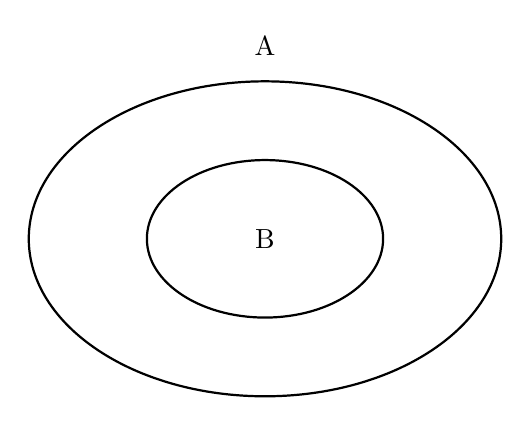
\begin{tikzpicture}
                            \draw[thick] (0,0) ellipse (3cm and 2cm);
                            \draw[thick] (0,0) ellipse (1.5cm and 1cm);

                            \node[above=2mm] at (0,2cm) {A};
                            \node at (0,0) {B};

                        \end{tikzpicture}
                        }
                    \end{latin}

                    \renewcommand{\thefigure}{1.1}
                    \caption{مجموعه $B$ زیر مجموعه مجموعه $A$ باشد.}
                \end{figure}
            
            \subsubsection*{(ج)}
                \[A = {a, b, c, d}, B = {a},\]
                $P(A) = \{\emptyset, \{a\}, \{b\}, \{c\}, \{d\}, \{a, b\}, \{a, c\}, \{a, d\}, \{b, c\}, \{b, d\}, \{c, d\}, \\ \{a, b, c\}, \{a, b, d\}, \{a, c, d\}, \{b, c, d\}, \{a, b, c, d\}\}$\\
                \[P(B) = \{\emptyset, \{a\}\}\]
                \[\rightarrow P(A:B) = \{X \in P(A) | B \subseteq X\} \Rightarrow \]
                \[P(A:B) = \{\{a\}, \{a, b\}, \{a, c\}, \{a, d\}, \{a, b, c\}, \{a, b, d\}, \{a, c, d\}, \{a, b, c, d\}\}\]

        \subsection*{جواب سوال نهم : }
            \subsubsection*{(الف)}
                \[P(\bigcap_{X \in \beta} X) = \bigcap_{X \in \beta} P(X) \rightarrow \]
                \[(P(\bigcap_{X \in \beta} X) \subseteq \bigcap_{X \in \beta} P(X)) \land (\bigcap_{X \in \beta} P(X) \subseteq \bigcap_{X \in \beta} X))\]
                حال به اثبات $P(\bigcap_{X \in \beta} X) \subseteq \bigcap_{X \in \beta} P(X)$ میپردازیم :
                \[Y \in P(\bigcap_{X \in \beta} X) \Rightarrow Y \subseteq \bigcap_{X \in \beta} X\]
                از آنجایی $\forall X \in \beta : \bigcap X \subseteq X$ پس داریم :
                \[Y \subseteq X \rightarrow Y \in P(X)\]
                از آنجایی که $\forall X \in \beta : \bigcap P(X) \subseteq P(X)$ پس داریم :
                \[Y \in \bigcap_{X \in \beta} P(X)\]

            \subsubsection*{(ب)}
                \[\bigcup_{X \in \beta} P(X) \subseteq P(\bigcup_{X \in \beta} X) \rightarrow \]
                \[Y \in \bigcup_{X \in \beta} P(X) \Rightarrow Y \subseteq \bigcup_{X \in \beta} X \Rightarrow Y \in P(\bigcup_{X \in \beta} X) \rightarrow\]
                \[\bigcup_{X \in \beta} P(X) \subseteq P(\bigcup_{X \in \beta} X)\]

        \subsection*{جواب سوال دهم : }
            \subsubsection*{(الف)}
                \[\bigcap_{i \in I} (X - X_i) = X - \bigcap_{i \in I} X_i \rightarrow\]
                \[(\bigcap_{i \in I} (X - X_i) \subseteq X - \bigcap_{i \in I} X_i) \land (X - \bigcap_{i \in I} X_i \subseteq \bigcap_{i \in I} (X - X_i))\]
                حال به اثبات $\bigcap_{i \in I} (X - X_i) \subseteq X - \bigcap_{i \in I} X_i$ میپردازیم :
                \[Y \in \bigcap_{i \in I} (X - X_i) \rightarrow \forall i \in I : (Y \in X - X_i) \rightarrow\]
                \[\forall i \in I : (Y \in X \land Y \not \in X_i) \rightarrow Y \in X \land \forall i \in I : (Y \not \in X_i) \rightarrow\]
                \[Y \in X \land Y \in \bigcup_{i \in I} X_i \rightarrow Y \in X - \bigcup_{i \in I} X_i\]
            
            \subsubsection*{(ب)}
                \[X - \bigcap_{i \in I} X_i = \bigcup_{i \in I} (X - X_i) \rightarrow\]
                \[(X - \bigcap_{i \in I} X_i \subseteq \bigcup_{i \in I} (X - X_i)) \land (\bigcup_{i \in I} (X - X_i) \subseteq X - \bigcap_{i \in I} X_i)\]
                حال به اثبات $X - \bigcap_{i \in I} X_i \subseteq \bigcup_{i \in I} (X - X_i)$ میپردازیم :
                \[Y \in X - \bigcap_{i \in I} X_i \rightarrow Y \in X \land Y \not \in \bigcap_{i \in I} X_i \rightarrow\]
                \[Y \in X \land \forall i \in I : (Y \not \in X_i) \rightarrow \forall i \in I : (Y \in X \land Y \not \in X_i) \rightarrow\]
                \[\forall i \in I : (Y \in X - X_i) \rightarrow Y \in \bigcup_{i \in I} (X - X_i)\]

        \subsection*{جواب سوال یازدهم : }
            \[\bigcap_{n=2}^{\infty} A_n\]
            چون با میل کردن $n$ به بینهایت بازه $A_n$ بزرگتر میشود، پس اشتراک همه این بازه های $A_2$ تا $A_n$, $A_2$ میشود :
            \[\bigcap_{n=2}^{\infty} A_n = A_2 = (0, \frac{1}{2})\]

            \[\bigcap_{n=2}^{\infty} B_n\]
            از آنجا که با میل کردن $n$ به بینهایت، بازه $B_n$، کوچکتر میشود داریم :
            \[\bigcap_{n=2}^{\infty} B_n = \lim_{n \to \infty} B_n = \emptyset\]

            \[\bigcup_{n=2}^{\infty} A_n\]
            \[\bigcup_{n=2}^{\infty} A_n = \lim_{n \to \infty} A_n = (0, 1)\]

            \[\bigcup_{n=2}^{\infty} B_n\]
            \[\bigcup_{n=2}^{\infty} B_n = B_2 = (\frac{1}{2}, 1)\]

        \subsection*{جواب سوال دوازدهم : }
            \[A_n = (2 - \frac{1}{n}, 2 + \frac{1}{n}), F = {n \in \mathbb{N} | A_n} = \{(1, 3), (1.5, 2.5), ..., \emptyset\} \rightarrow\]
            \[\bigcup_{B \in F} B = A_1 = (1, 3)\]
            \[\bigcap_{B \in F} B = \lim_{n \to \infty} A_n = \emptyset\]

\end{document}